\subsection{2-dimensional DP}
We illustrate the two approaches using a simple grid problem.

You are asked to find the minimal-cost path from the top-left corner to the bottom-right corner of the grid.
You can only walk right and down to adjacent tiles. The cost of the path equals the sum of the values of the tiles you walk through.

It is easy to see that the cost to reach a tile is equal to the value of the tile plus the cost to reach the tile on top of it or plus the cost to reach the tile left of it.
Figure~\ref{image:2d-problem} show the problem. Figure~\ref{image:2d-solution} shows for every tile the cost to get there.

\begin{figure}
\label{image:2d-problem}
 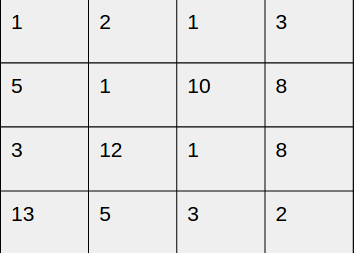
\includegraphics{2d/problem.png}
 \caption{The grid with on each tile the cost to walk through it.}
\end{figure}
\begin{figure}
  \label{image:2d-solution}
 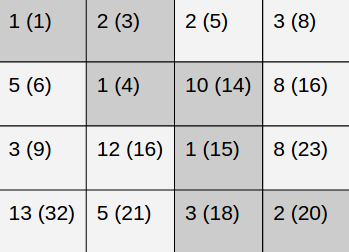
\includegraphics{2d/solution.png}
 \caption{The grid with on each tile the cost to walk through it and between brackets the cheapest way to get there (cost to walk throught the tile itself included).}
\end{figure}

The first algorithm shows the top-down approach. 
Whenever we need the cost to reach a certain tile, it checks whether the cost has been calculated.
If this is not the case, it calculates the solution for this tile.
If the cost was calculated earlier, it just uses the previously calculated value.
The code is shown in Listing~\ref{code-2d-1}.
\lstinputlisting[label=code-2d-1,caption=Top-down approach, language=C++,firstline=8, lastline=20, tabsize=2, breaklines=true, numbers=left, float]{src/2d/topdown.cpp}

The second algorithm shows the bottom-up approach.
We first populate the top row and left column of the table. 
Next, the algorithm fills all elements in the table row per row from left to right.
In this step, it uses the values of the tile on top of the current tile and the tile left of the current tile.
The code is shown in Listing~\ref{code-2d-2}.
\lstinputlisting[label=code-2d-2,caption=Bottom-up approach, language=C++,firstline=8, lastline=18, tabsize=2, breaklines=true, numbers=left, float]{src/2d/bottomup.cpp}